\documentclass[]{article}

\usepackage{fontenc}
\usepackage{array}
\usepackage[bottom=2.5cm, left=2.5cm, right=2.5cm, top=2.5cm]{geometry}
\usepackage{tabularx}
\usepackage{graphicx}
\usepackage{siunitx}
\usepackage{booktabs}
\usepackage[]{hyperref}
\usepackage[]{natbib}
\usepackage{authblk}
\usepackage[usenames,dvipsnames]{xcolor}

\definecolor{forestgreen}{rgb}{0.13, 0.55, 0.13}

\hypersetup{
    linkcolor=red,
    citecolor=forestgreen,
    colorlinks=true,
    pdfborder={0 0 0}
}

\renewcommand{\thesection}{SI \arabic{section}}
\makeatletter
\renewcommand\@maketitle{%
{\noindent\sffamily\Large\bfseries{\@title} \par }
\vspace{10pt}
{\noindent\@author \par}
\vspace{0.5cm}
{\noindent\textit{Correspondence to: }{Ga\"{e}lle Uzu (gaelle.uzu@ird.fr)}}
}
\makeatother

\title{An apportionment method for the Oxydative Potential to the atmospheric PM
sources: application to a one-year study in Chamonix, France.\\ Suplementary
Informations}

\author[1]{Weber, Samu\"{e}l}
\author[1]{Uzu, Ga\"{e}lle}
\author[1]{Calas, Aude}
\author[1,2]{Chevrier, Florie}
\author[2]{Besombes, Jean-Luc}
\author[1,3]{Charon, Aur\'{e}lie}
\author[1]{Salameh, Dalia}
\author[4]{Je\v{z}ek, Irena}
\author[4,5]{Mo\v{c}nik, Gri\v{s}a}
\author[1]{Jaffrezo, Jean-Luc}

\affil[1]{Univ. Grenoble Alpes, CNRS, IRD, IGE (UMR 5001), F-38000 Grenoble, France.}
\affil[2]{Univ. Savoie Mont-Blanc, LCME, F-73 000 Chamb\'{e}ry, France.}
\affil[3]{IFFSTAAR, F-69675 Bron, France.}
\affil[4]{Aerosol d.o.o., Kamni\v{s}ka 41, 1000 Ljubljana, Slovenia.}
\affil[5]{Condensed Physics Department, Jo\v{z}ef Stefan Institute, Ljubljana, Slovenia.}

% \runningtitle{Apportionment of OP sources in Chamonix, France}
%
% \runningauthor{Weber et al.}
%
% \correspondence{Ga\"{e}lle Uzu (gaelle.uzu@ird.fr)}




\begin{document}

% \firstpage{1}

\maketitle
\linespread{1.2}\selectfont

\section{Sources profiles from the PMF}
\label{si-1-sources-profiles-from-the-pmf}

\begin{description}
    \item[Biomass burning] is a profile highly represented by biomass
        burning proxy: the levoglucosan and the methoxyphenols. The
        BC\textsubscript{bb} and OC* are also mainly in this factor. Associated
        with it, some potassium and rubidium are also present in this source.
        These proxy are well-known to be tracers of biomass burning activities
        \citep{godoy_aerosol_2005,jordan_levoglucosan_2006,nava_biomass_2015,puxbaum_levoglucosan_2007}

    \item[Vehicular emissions] are associated to a very large contribution
        of metals (Cu, Mo, Pb, Sb, Fe, Zr, Ti) and a significant amount of
        carbonaceous matter (mainly BC\textsubscript{ff}) and organic compound
        (HOP). The two sources from vehicle' traffic which are ``exhaust'' (i.e.
        fuel combustion \citep{allen_size_2001,hu_metals_2009,viana_source_2008}) and ``non-exhaust'' (i.e. road abrasion, brake wear, etc.
        \citep{sanders_airborne_2003,sternbeck_metal_2002}) are mixed in this
        profile.

    \item[Primary biogenic] emissions are identified thanks to the
        presence of polyols (sum of arabitol, sorbitol and mannitol) coming from
        the biogenic activity (fungi, pollens and bacteria) (Bauer et al., 2008)
        or from vegetal debris \citep{yttri_ambient_2007}. The temporal contribution
        of this factor (mainly during summer) also pledges in favour of the
        biogenic activity.

    \item[Secondary biogenic emissions] are dominated by the MSA (methane
        sulfonic acid), product by the oxidation of the DMS (dimethyl sulfate).
        The DMS is well-known for being emitted by marine algae
        \citep{saltzman_methane_1983,zhang_surface_2014} or vegetation and soil
        micro-biology \citep{jardine_dimethyl_2015}.

    \item[Crustal dust] is characterized with a high predominance of
        Mg\textsuperscript{2+}, Ca\textsuperscript{2+}, Ti, Mn, Fe, which are
        elements of the terrestrial crust. We identified this source as
        re-suspension of soil or rock dust
        \citep{almeida_source_2005,dallosto_hourly_2013,moreno_variations_2011,putaud_size-segregated_2004}.

    \item[Sea/road salt] shows a high proportion of Na\textsuperscript{+}
        and Cl\textsuperscript{-}, but also Mg\textsuperscript{2+}. These ions
        are proxy of sea salt
        \citep{belis_critical_2013,odowd_marine_1997,pio_climatology_2007} as well as road salt, especially during winter in the Alps
        region \citep{air_rhone-alpes_influence_2012}.

    \item[Nitrate rich] with a high concentration of nitrate ions
        (NO\textsubscript{3}\textsuperscript{-}) associates with ammonium
        (NH\textsubscript{4}\textsuperscript{+}). It indicates the presence of
        ammonium nitrate NO\textsubscript{3}NH\textsubscript{4}.

    \item[Sulfate rich] with a high concentration of sulfate ions
        (SO\textsubscript{4}\textsuperscript{2-}) associates with ammonium
        (NH\textsubscript{4}\textsuperscript{+}). It indicates the presence of
        ammonium sulfate
        SO\textsubscript{4}(NH\textsubscript{4})\textsubscript{2}.

\end{description}

Table~\ref{tab:concPerg} summaries the factor profiles in~\SI{1}{{\mu}g} of PM
of each source while Fig.~\ref{fig:concPercent} presents the fraction of each
species associated with each source.

\begin{table}
    \centering
    \caption{Concentration of species in \SI{1}{{\mu}g} of PM for each source attributed by the PMF model.}
    \footnotesize
    \begin{tabularx}{\textwidth}{lSSSSSSSSS}
        \toprule
        specie & 
        \multicolumn{1}{X}{Primary\newline biogenic} & 
        \multicolumn{1}{X}{Sea/road\newline salt} &
        \multicolumn{1}{X}{Secondary\newline biogenic} &
        \multicolumn{1}{X}{Crustal\newline dust} &
        \multicolumn{1}{X}{Vehicular} & 
        \multicolumn{1}{X}{Biomass\newline burning} & 
        \multicolumn{1}{X}{Nitrate\newline rich} &
        \multicolumn{1}{X}{Sulfate\newline rich}\\
        \midrule
        \multicolumn{9}{c}{\si{ng\per{\mu}g}}\\
        \midrule
        OC* & 412.86 & 228.75 & 733.01 & 180.92 & 301.20 & 401.67 & 225.14 & 249.95\\
        BC\textsubscript{bb} & 15.37 & 19.29 & 22.65 & 4.35 & 24.69 & 72.99 & 10.96 & 6.91\\
        BC\textsubscript{ff} & 160.58 & 72.08 & 116.95 & 8.35 & 295.70 & 0 & 63.05 & 0.48\\
        MSA & 0.27 & 0 & 18.38 & 0 & 0.07 & 0 & 0.37 & 0.09\\
        Cl\textsuperscript{-} & 0 & 36.48 & 0 & 0 & 0 & 4.74 & 4.35 & 0\\
        NO\textsubscript{3}\textsuperscript{-} & 4.58 & 0 & 71.42 & 102.12 & 0 & 9.41 & 427.27 & 18.97\\
        SO\textsubscript{4}\textsuperscript{2-} & 26.33 & 20.65 & 37.48 & 72.18 & 0 & 39.76 & 0 & 302.41\\
        Na\textsuperscript{+} & 3.07 & 62.22 & 21.23 & 0.09 & 2.80 & 1.52 & 0 & 0.62\\
        NH\textsubscript{4}\textsuperscript{+} & 11.47 & 4.25 & 0 & 0 & 6.02 & 8.82 & 86.69 & 108.24\\
        K\textsuperscript{+} & 9.11 & 3.96 & 10.18 & 3.70 & 2.21 & 9.53 & 3.33 & 3.33\\
        Mg\textsuperscript{2+} & 0.15 & 0.68 & 2.86 & 4.43 & 0 & 0.39 & 0 & 0.52\\
        Ca\textsuperscript{2+} & 0 & 0 & 11.74 & 115.47 & 5.62 & 3.07 & 8.54 & 11.97\\
        Levoglucosan & 8.07 & 21.00 & 2.37 & 0 & 13.77 & 107.71 & 32.88 & 4.64\\
        $\Sigma$polyols & 14.55 & 0 & 3.27 & 1.09 & 0 & 0.64 & 0.43 & 1.66\\
        $\Sigma$methoxy & 0 & 0 & 0 & 0.60 & 0 & 11.34 & 0 & 0\\
        Fe & 12.14 & 21.73 & 8.04 & 38.82 & 42.06 & 1.02 & 0 & 1.00\\
        \midrule
        \multicolumn{9}{c}{\si{pg\per{\mu}g}}\\
        \midrule
        As & 16.16 & 2.32 & 55.47 & 37.70 & 64.14 & 0.00 & 12.97 & 16.55\\
        Cu & 552.51 & 421.26 & 908.64 & 261.28 & 1147.23 & 247.42 & 0 & 92.72\\
        Mn & 150.02 & 146.43 & 381.62 & 1224.90 & 495.22 & 21.15 & 4.25 & 140.64\\
        Mo & 17.22 & 16.99 & 39.99 & 13.09 & 82.84 & 0 & 0 & 13.62\\
        Ni & 4.17 & 21.56 & 0.13 & 106.58 & 46.94 & 0 & 0 & 18.64\\
        Pb & 75.42 & 0 & 119.94 & 156.67 & 380.18 & 0 & 99.35 & 113.36\\
        Rb & 11.03 & 18.15 & 0 & 69.91 & 34.72 & 27.09 & 0 & 0\\
        Sb & 25.32 & 28.88 & 27.92 & 0 & 80.69 & 0 & 6.15 & 3.11\\
        Ti & 308.11 & 135.57 & 253.05 & 1754.87 & 291.41 & 0 & 42.31 & 101.03\\
        V & 28.44 & 21.14 & 31.64 & 92.69 & 0 & 0 & 0 & 14.14\\
        Zn & 377.67 & 225.73 & 1240.86 & 548.98 & 2091.33 & 139.94 & 602.30 & 373.39\\
        Zr & 45.51 & 11.33 & 16.67 & 34.12 & 52.09 & 6.24 & 6.56 & 0\\
        $\sigma$HOP & 0 & 145.45 & 4.77 & 8.66 & 140.33 & 0.00 & 34.46 & 0\\
        \bottomrule
    \end{tabularx}
    \label{tab:concPerg}
\end{table}

\begin{figure}[h]
    \centering
    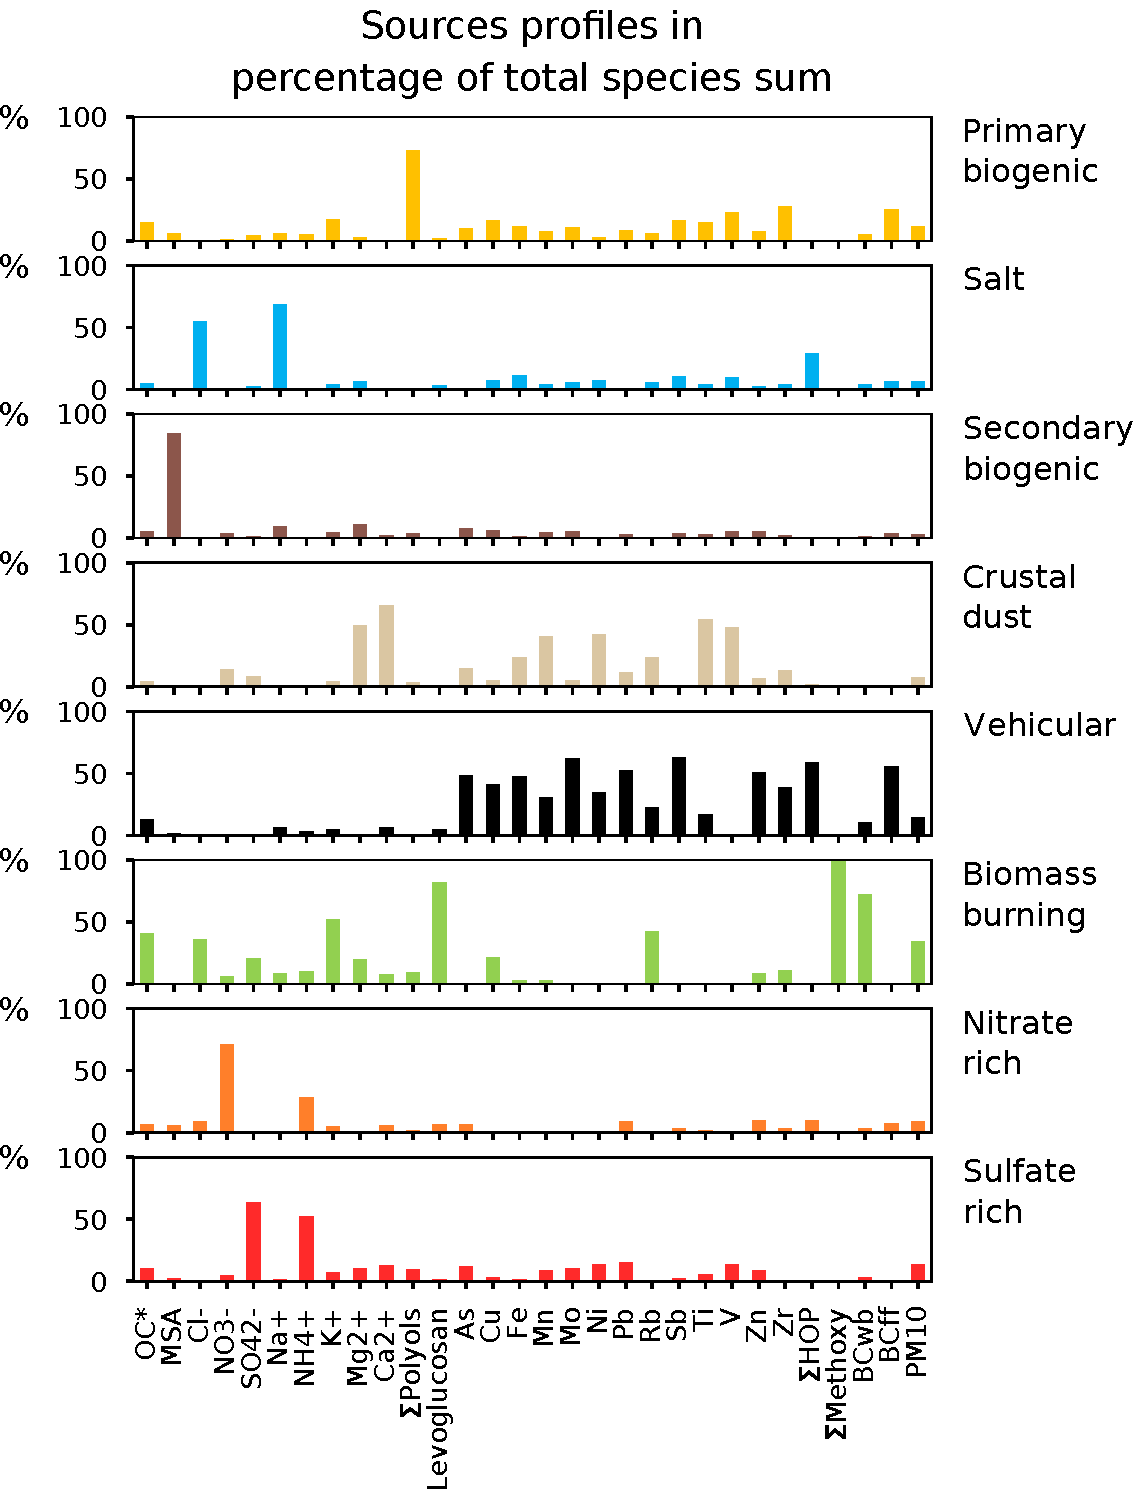
\includegraphics[width=0.8\textwidth]{figures/SI_fig01}
    \caption{Percentage of the ambient species concentration apportioned in each
        factor attributed by the PMF model.}
    \label{fig:concPercent}
\end{figure}
\clearpage

\section{Correlation between OP and chemical species, and OP and
sources}\label{si-2-correlation-between-op-and-chemical-species-and-op-and-sources}

The univariate correlation on an annual basis between the OP values and the
concentrations of chemical species was first investigated and is presented in
Fig.~\ref{fig:pearsonrChem}. We see a strong relationship between some of the
organic species and the OP (levoglucosan, methoxyphenol) as well as the
carbonaceous matter (OC and BC) for both tests. It suggests important
contributions of biomass burning source and fossil fuel burning activities to
the OP's. The metals Cu, Rb, and Sb appear highly correlated to the OP, but Ni,
Ti and V do not. The results for the ions indicate weak positive correlations
with both OP only. We also note that the polyols and MSA show a tendency with
anti-correlations with both OPs. Most of these results are strongly affected by
the really high changes in concentrations during the winter and the summer
periods, in part related to the local impact of meteorology and inversion layers
in winter \citep{calas_comparison_2018}.

\begin{figure}[h]
    \centering
    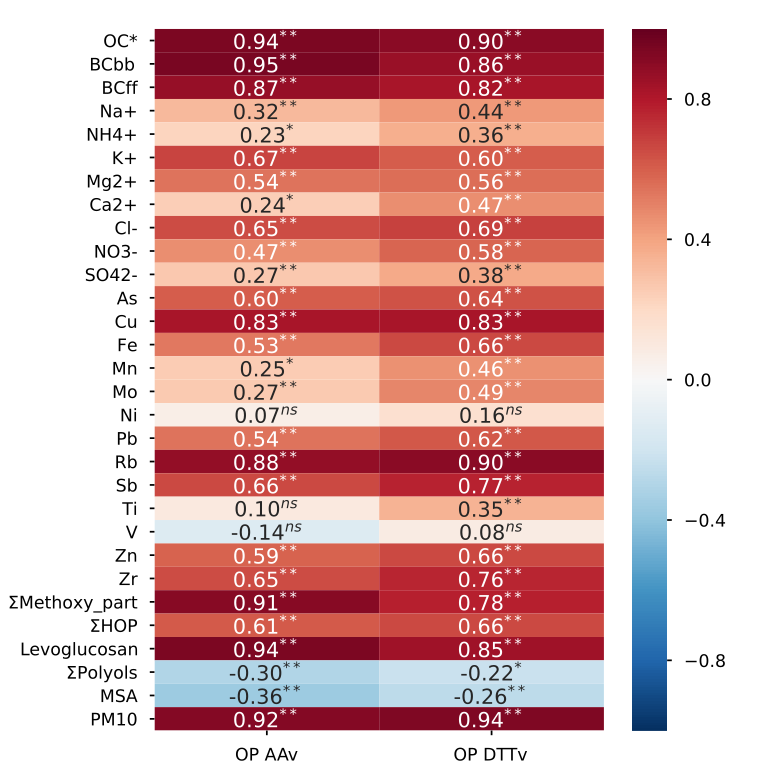
\includegraphics[width=0.7\textwidth]{figures/SI_fig02}
    \caption{Pearson's correlation coefficient between the concentrations of the
        species and the OP AA\textsubscript{v} and OP DTT\textsubscript{v}
        activity from the 2, November 2013 to the 31, October 2014 (97 samples).
        **: p-values \textless{}0.01, *: p-value \textless{}0.05, ns: p-value
    \textgreater{}0.05.}
    \label{fig:pearsonrChem}
\end{figure}

The univariate-correlation between the contributions of the sources of PM
deduced from the PMF and the OPs is presented Fig.~\ref{fig:pearsonrSrc}. It
emphasized the hypothesis of the high contribution of the biomass burning and
vehicular sources to the OP of the PM\textsubscript{10}. We do not see very
large differences between the two tests, expect for the crustal dust source (no
correlation with the OP AA\textsubscript{v} but a positive one for the OP
DTT\textsubscript{v}).

\begin{figure}[h]
    \centering
    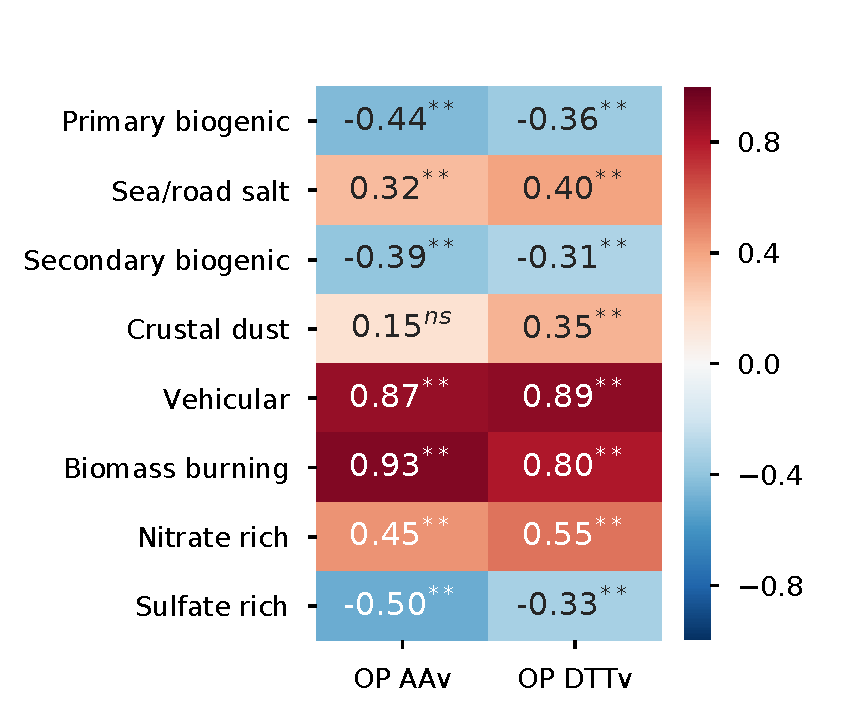
\includegraphics[width=0.6\textwidth]{figures/SI_fig03}
    \caption{Pearson's correlation coefficient between the PM concentrations of
        the sources from the PMF and the OP AA\textsubscript{v} and OP
        DTT\textsubscript{v} activity from the 14, November 2013 to the 31,
        October 2014 (85 samples). **: p-values \textless{}0.01, *: p-value
    \textless{}0.05, ns: p-value \textgreater{}0.05.}
    \label{fig:pearsonrSrc}
\end{figure}
\clearpage

\section{Additional reference}\label{additional-reference}
\bibliographystyle{copernicus}
\bibliography{bibtex}


\end{document}
